\section{Background}
\label{background}

As touched upon in section ~\ref{introduction}, locality-sensitive hashing tackles the problem of similarity search in high-dimensional datasets by relaxing the requirement of finding exact nearest neighbours. Instead, LSH is used as an \textit{approximate} nearest neighbour algorithm, which inherently implies only probabilistic guarantees of finding a nearest neighbour. In general, LSH act as a randomized filter that attempts to reduce an input set to a subset of candidates for a given query item.

The LSH schemes considered in this paper both operate in so-called \textit{Hamming space}:

\begin{definition}
\label{definition-hamming-space}
  A Hamming space $H(d, a)$ is the set of all words of length $d$ over an alphabet of size $a$. A distance measure over a Hamming space is the number of letters in which two words differ.
\end{definition}

The alphabet that we consider for LSH is $\{0, 1\}$ and words are therefore bit vectors of $d$ dimensions. The definition of the approximate nearest neighbour problem for Hamming space is given as follows in \cite{DBLP:journals/corr/PhamP16}:

\begin{definition}
\label{definition-nearest-neighbour}
  Given a set of vectors of dimensionality $d$ $Z \subset \{0, 1\}^d$, $|Z| = n$, the Hamming distance function $D$, a radius $r > 0$, an approximation factor $c > 1$, and a false negative rate $\delta > 0$, construct a data structure such that, given any query $q \in \{0,1\}^d$, if there exists $x \in Z$ and $D(x, q) \leq r$, it reports some $y \in Z$ where $D(y, q) \leq cr$ with probability $1 - \delta$.
\end{definition}

The data structure mentioned in definition ~\ref{definition-nearest-neighbour} makes use of a family of \textit{locality-sensitive hash functions} in order to hash items to buckets. The definition of this family is given as follows in \cite{DBLP:conf/stoc/IndykM98}:

\begin{definition}
\label{definition-hash-functions}
  Given $r$, $c$, and probabilities $p_1$ and $p_2$ where $p_1 < p_2$, a family $H$ is said to be $(r, cr, p_1, p_2)$-sensitive for $(Z, D)$ if for any $x, y \in Z$ we have

  \begin{itemize}
    \item if $D(x, y) \leq r$ then $Pr_H [h(x) = h(y)] \geq p_1$,
    \item if $D(x, y) > cr$ then $Pr_H [h(x) = h(y)] \leq p_2$.
  \end{itemize}
\end{definition}

Here, $p_1$ is the lower bound on the probability of close vectors colliding and $p_2$ is the upper bound on the probability of distant vectors colliding \cite[p. 100]{DBLP:books/cu/LeskovecRU14}. We therefore want $p_1$ to be close to 1 and $p_2$ to be close to 0.

\subsection{Classic LSH}
\label{background-classic-lsh}

The classic LSH family for Hamming space uses a random bit sampling approach for picking a number of components from an input vector. This sample is then used as the key in a map structure, which will be referred to as a \textit{partition}, for locating a bucket that the vector should be stored in. The bits to sample for a given partition are chosen independently and uniformly at random and stored with the partition. When looking for the nearest neighbour of a query vector, this sampling is repeated and the candidate vectors are those found in the bucket that the sample maps to.

\begin{example}
\label{example-classic-sampling}
  Given input vector $v = 1101$, we randomly chose to sample component 1 and 3, giving us the key $v' = 10$. We then proceed to update our map structure with an entry for this key: $10 \rightarrow \{1101\}$

  Given another input vector $u = 0110$, we again sample component 1 and 3, giving us the key $u' = 01$. We then add another entry to our map: $10 \rightarrow \{1101\}, 01 \rightarrow \{0110\}$.

  Given a query vector $q = 1001$, we once again sample component 1 and 3, giving us the key $q' = 10$. We then look up this key in our map and receive the following set of candidates: $\{1101\}$.
\end{example}

\begin{figure}[ht]
  \centering
  \begin{tikzpicture}
    \node (u) {u = \underline{0}1\underline{1}0};
    \node (v) [right=of u] {v = \underline{1}1\underline{0}1};
    \node (q) [right=of v] {q = \underline{1}0\underline{0}1};

    \matrix (m) [matrix of nodes, below=of v, row sep=-\pgflinewidth, style={nodes={draw}}]{
    01 & 10 & 11 \\
    };

    \path [->] (u.east) edge [bend left=30] ([yshift=0.5ex] m-1-1.north);
    \path [->] (v.south) edge ([yshift=0.5ex] m-1-2.north);
    \path [->] (q.west) edge [bend right=30] ([yshift=0.5ex, xshift=0.5ex] m-1-2.north);
  \end{tikzpicture}

  \caption{A graphical depiction of example ~\ref{example-classic-sampling}}
  \label{figure-classic-sampling}
\end{figure}

As can be seen in example ~\ref{example-classic-sampling}, $v$ and $u$ are not particularly similar as they only share a single component; by the sampling 1 and 3 they therefore do not map to the same bucket. However, $v$ and $q$ are almost identical as they share all but one component; the sampling 1 and 3 therefore maps them to the same bucket, albeit by chance. We have effectively reduced the set of potential candidates to half of the items in the original input set.

By adjusting the number of components sampled from vectors we can change the probability of collisions happening in the data structure. That is, by increasing the sample size we decrease the chance of vectors colliding, and vice versa, as more components would then have to match in order for a collision to happen.

If we want to keep the same sample size, but still increase the chance of vectors colliding, then we need to use more than one partition. Every partition will then independently chose the bits to sample and the set of candidate vectors will be the union of the vectors found in buckets in each partition.

\paragraph{Collision probabilities} By tweaking the sample size and the number of partitions to use, we can control the two probabilities $p_1$ and $p_2$ described in definition ~\ref{definition-hash-functions} \cite[p. 101]{DBLP:books/cu/LeskovecRU14}. By choosing a sample size $k$, the resulting probabilities will be $p_1^k$ and  $p_2^k$. On the other hand, by choosing a number of partitions 􏰄$l$, the resulting probabilities will be $1 - (1 - p_1)^l$ and $1 - (1 - p_2)^l􏰅$. By combining these, we get the probabilities $1 - (1 - p_1^k)^l$ and $1 - (1 - p_2^k)^l$, giving rise to what \cite[p. 89]{DBLP:books/cu/LeskovecRU14} calls the \textit{$S$-curve}:

\begin{figure}[ht]
  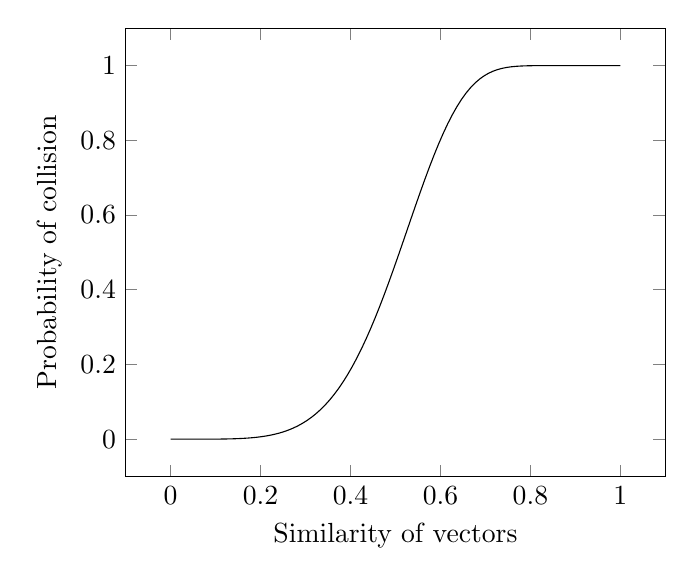
\begin{tikzpicture}
    \begin{axis}[
      xlabel = {Similarity of vectors},
      ylabel = {Probability of collision}
    ]
      \addplot[samples = 100, domain = 0:1]{1 - (1 - x^5)^20};
    \end{axis}
  \end{tikzpicture}

  \caption{The $S$-curve for $k = 5$, $l = 20$}
\end{figure}

\subsection{Covering LSH}
\label{background-covering-lsh}

Unlike the independently random bit sampling approach of classic LSH, covering LSH relies on a smarter sampling of correlated bits such that it can cover a given radius $r$. The difference between classic and covering LSH therefore lies in the family of hash functions used. The definition of a covering LSH family for Hamming space is given as follows in \cite{DBLP:journals/corr/PhamP16}:

\begin{definition}
\label{definition-covering-family}
  An LSH family $H$ is $r$-covering if for every two binary vectors $x, y \in \{0, 1\}^d$ with $D(x, y) \leq r$, there exists $h \in H$ such that $h(x) = h(y)$.
\end{definition}

A covering LSH family makes use of a random mapping $m \colon [d] \rightarrow \{0, 1\}^{r + 1}$ which constructs $d$ vectors, each consisting of $r + 1$ bits. This mapping is then used for constructing $2^{r + 1} - 1$ hash functions, or samplings, each associated with a different partition. In addition, each hash function is associated with a vector representation of $v \in \{1, \ldots, 2^{r + 1} - 1\}$. The bits to sample for each function in the family is determined by computing for each bit $b \in \{1, \ldots, d\}$, $m(b) \cdot v \bmod 2$, i.e. the dot product modulo 2 of $m(b)$ and $v$. If the result is 1, then the $b$th bit should be sampled.

\begin{example}
\label{example-covering-family}
  A 2-covering LSH family for $d = 4$ uses a random mapping $m \colon [4] \rightarrow \{0, 1\}^3$, e.g. $m(1) = 011, m(2) = 100, m(3) = 101, m(4) = 001$. This mapping is then used for constructing 7 hash functions, the first of which is $h(1)$:

  \begin{itemize}
    \item[] $b(1) = m(1) \cdot v \bmod 2 = 011 \cdot 001 \bmod 2 = 1$
    \item[] $b(2) = m(2) \cdot v \bmod 2 = 100 \cdot 001 \bmod 2 = 0$
    \item[] $b(3) = m(3) \cdot v \bmod 2 = 101 \cdot 001 \bmod 2 = 1$
    \item[] $b(4) = m(4) \cdot v \bmod 2 = 001 \cdot 001 \bmod 2 = 1$
  \end{itemize}

  $h(1)$ therefore samples bit 1, 3, and 4. This computation is repeated for the remaining hash functions, producing the following samplings:

  \begin{itemize}
    \item $h(2)$ samples bit 1
    \item $h(3)$ samples bit 3 and 4
    \item $h(4)$ samples bit 2 and 3
    \item $h(5)$ samples bit 1, 2, and 4
    \item $h(6)$ samples bit 1, 2, and 3
    \item $h(7)$ samples bit 2 and 4
  \end{itemize}
\end{example}

\begin{table}[h]
  \centering
  \begin{tabular}{c | c | c | c}
    & 1 & 2 & 3 \\
    \hline
    2 & $h(5)$, $h(6)$ & \cellcolor{gray!10} & \cellcolor{gray!10} \\
    \hline
    3 & $h(1)$, $h(6)$ & $h(4)$, $h(6)$ & \cellcolor{gray!10} \\
    \hline
    4 & $h(1)$, $h(5)$ & $h(5)$, $h(7)$ & $h(1)$, $h(3)$ \\
  \end{tabular}

  \caption{Depiction of how all possible combinations of 2 bits are covered by functions from the 2-covering family}
  \label{table-covering-family}
\end{table}

As can be seen from example ~\ref{example-covering-family}, which has been adapted from \cite[example 2.1]{DBLP:journals/corr/PhamP16}, and table ~\ref{table-covering-family}, a 2-covering LSH family for 4-dimensional vectors is able to "cover" all combinations of bit pairs. This in effect guarantees that no false negatives will be produced within the given radius of 2.

\paragraph{Constraints} The covering LSH family works under the assumption that $cr = \log n$. This constraint has in \cite{DBLP:journals/corr/Pagh15} been generalized to arbitrary values of $c$, $r$, and $n$ but we will not further touch upon these generalizations in this paper.
